\begin{landscape}
\begin{figure}

\centering{
    \begin{tabular}{c c c c}
        $M_\chi$ &
        $\chi\chi \rightarrow$ \parpar{b} &
        $\chi\chi \rightarrow$ \parpar{\tau} &
        $\chi\chi \rightarrow$ \parpar{\nu_\mu} \\

        \rotatebox[origin=c]{90}{1 TeV} &
        \raisebox{-.5\height}{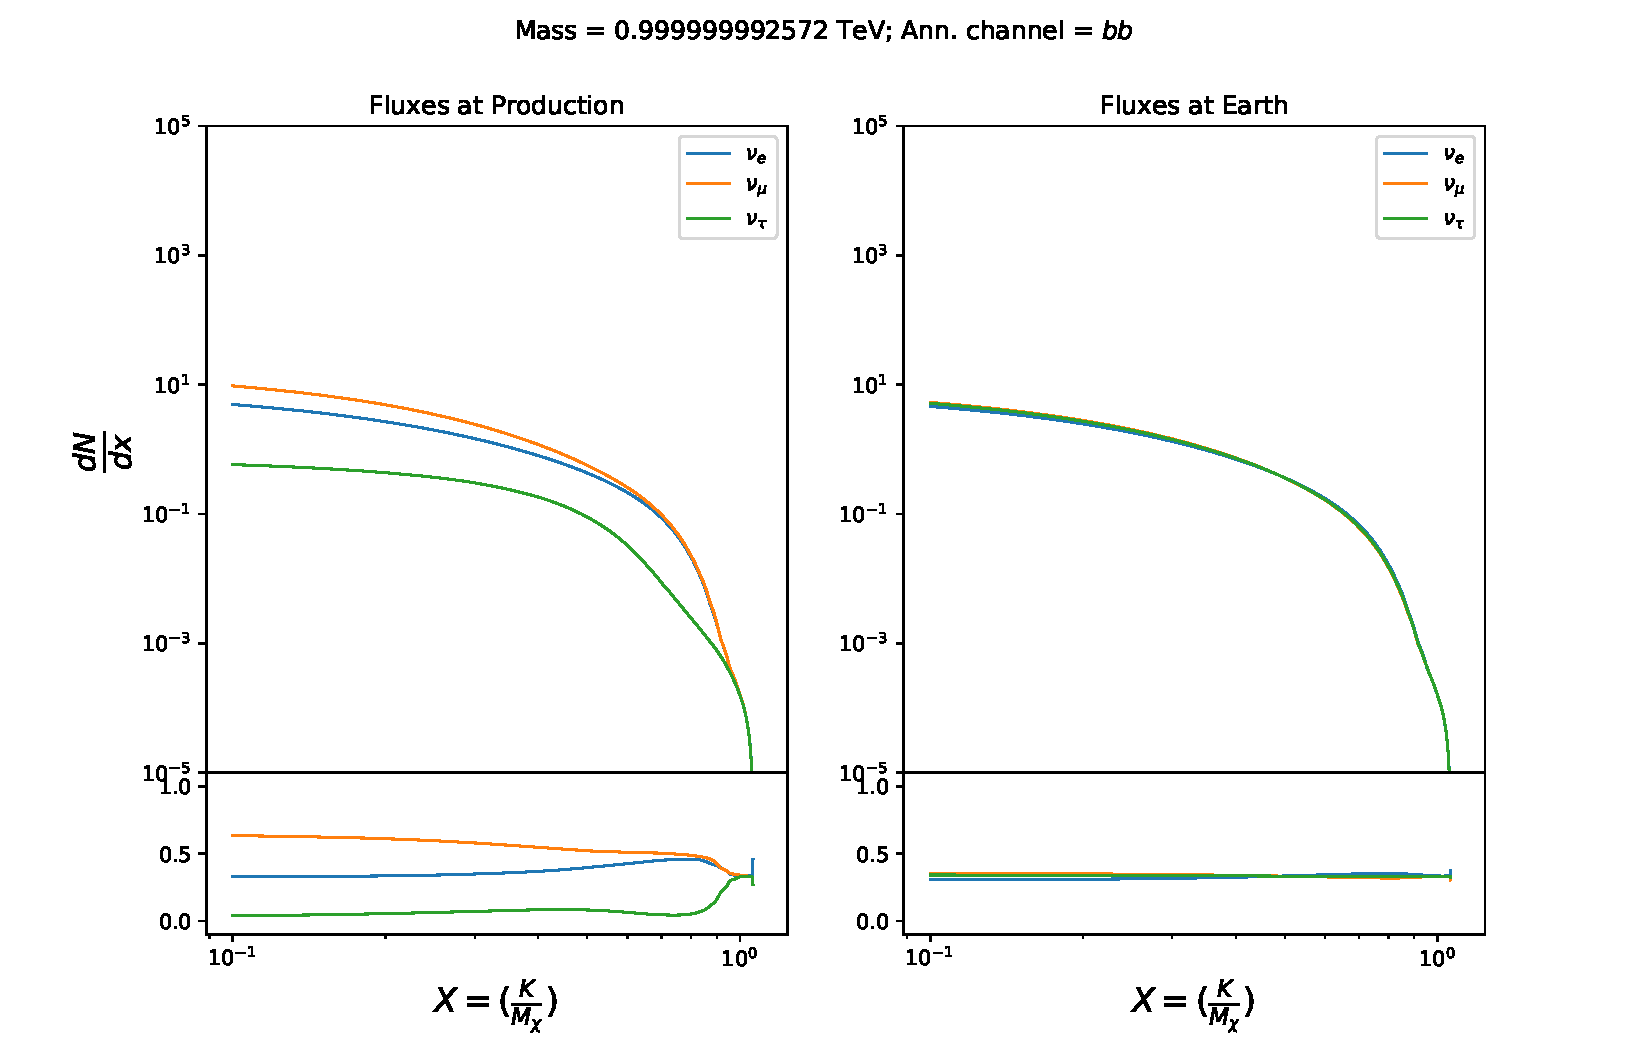
\includegraphics[clip, trim=1cm 0cm 2.5cm 1cm, scale=0.279]{figures/ic_DM/nu_spectra_bb_1.0000TeV.pdf}} &
        \raisebox{-.5\height}{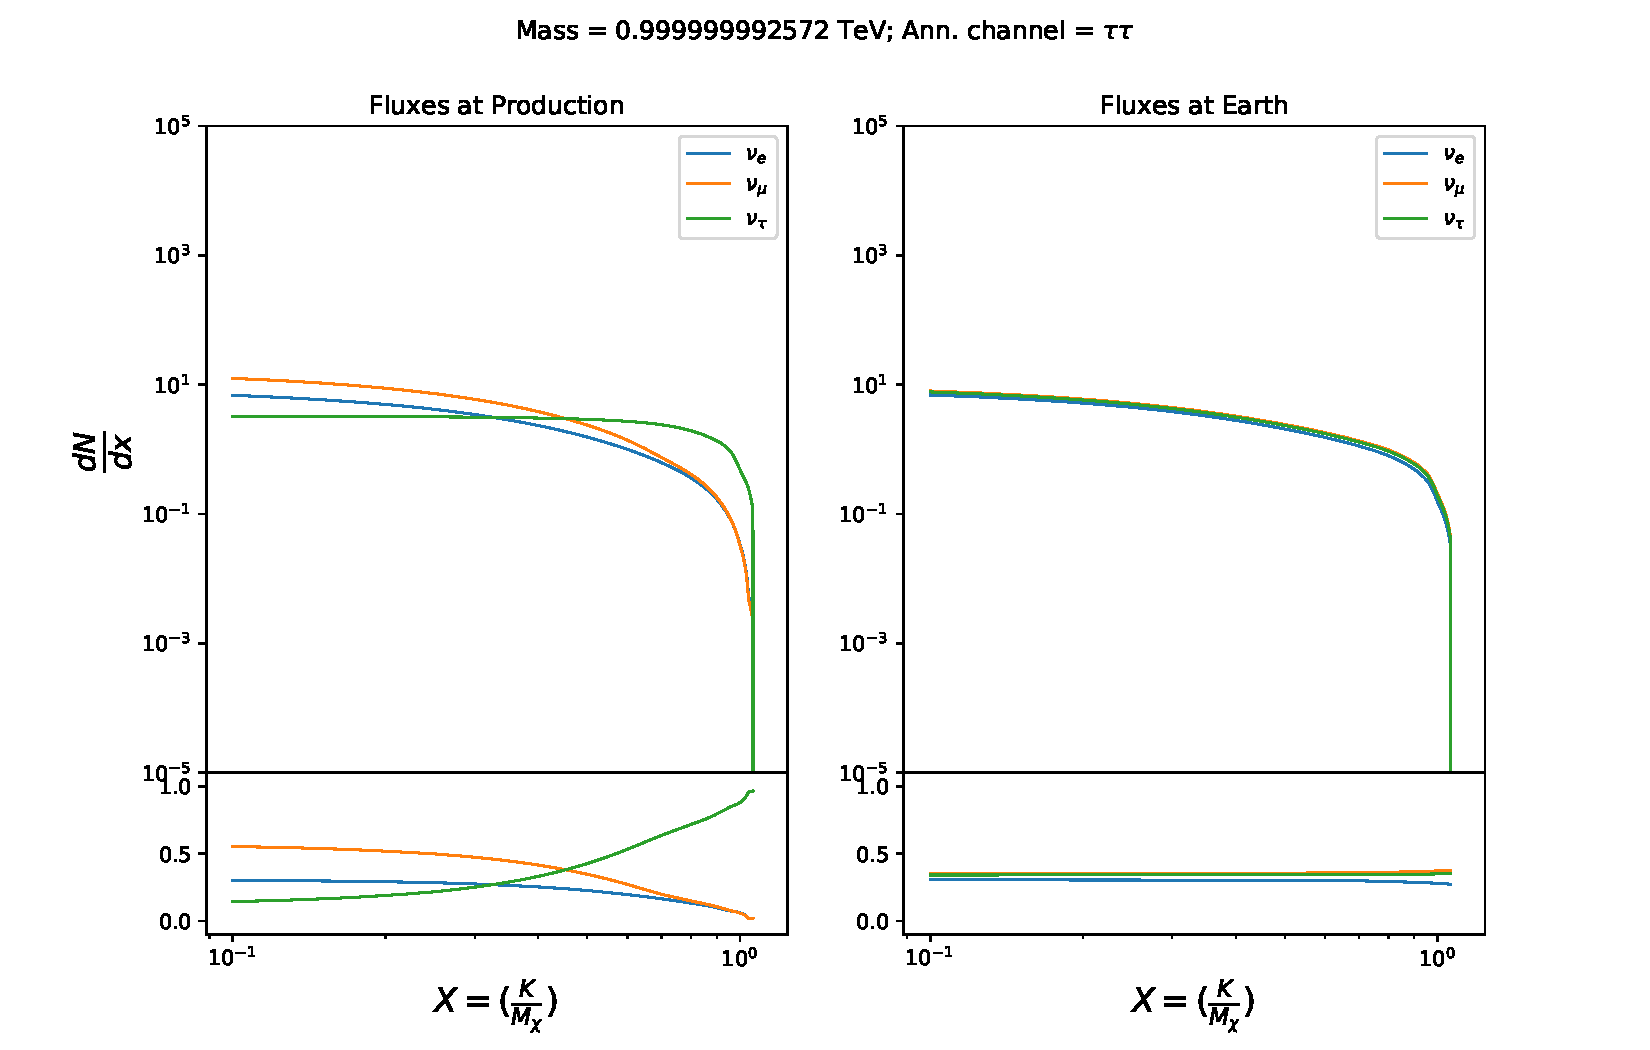
\includegraphics[clip, trim=1cm 0cm 2.5cm 1cm, scale=0.279]{figures/ic_DM/nu_spectra_tautau_1.0000TeV.pdf}} &
        \raisebox{-.5\height}{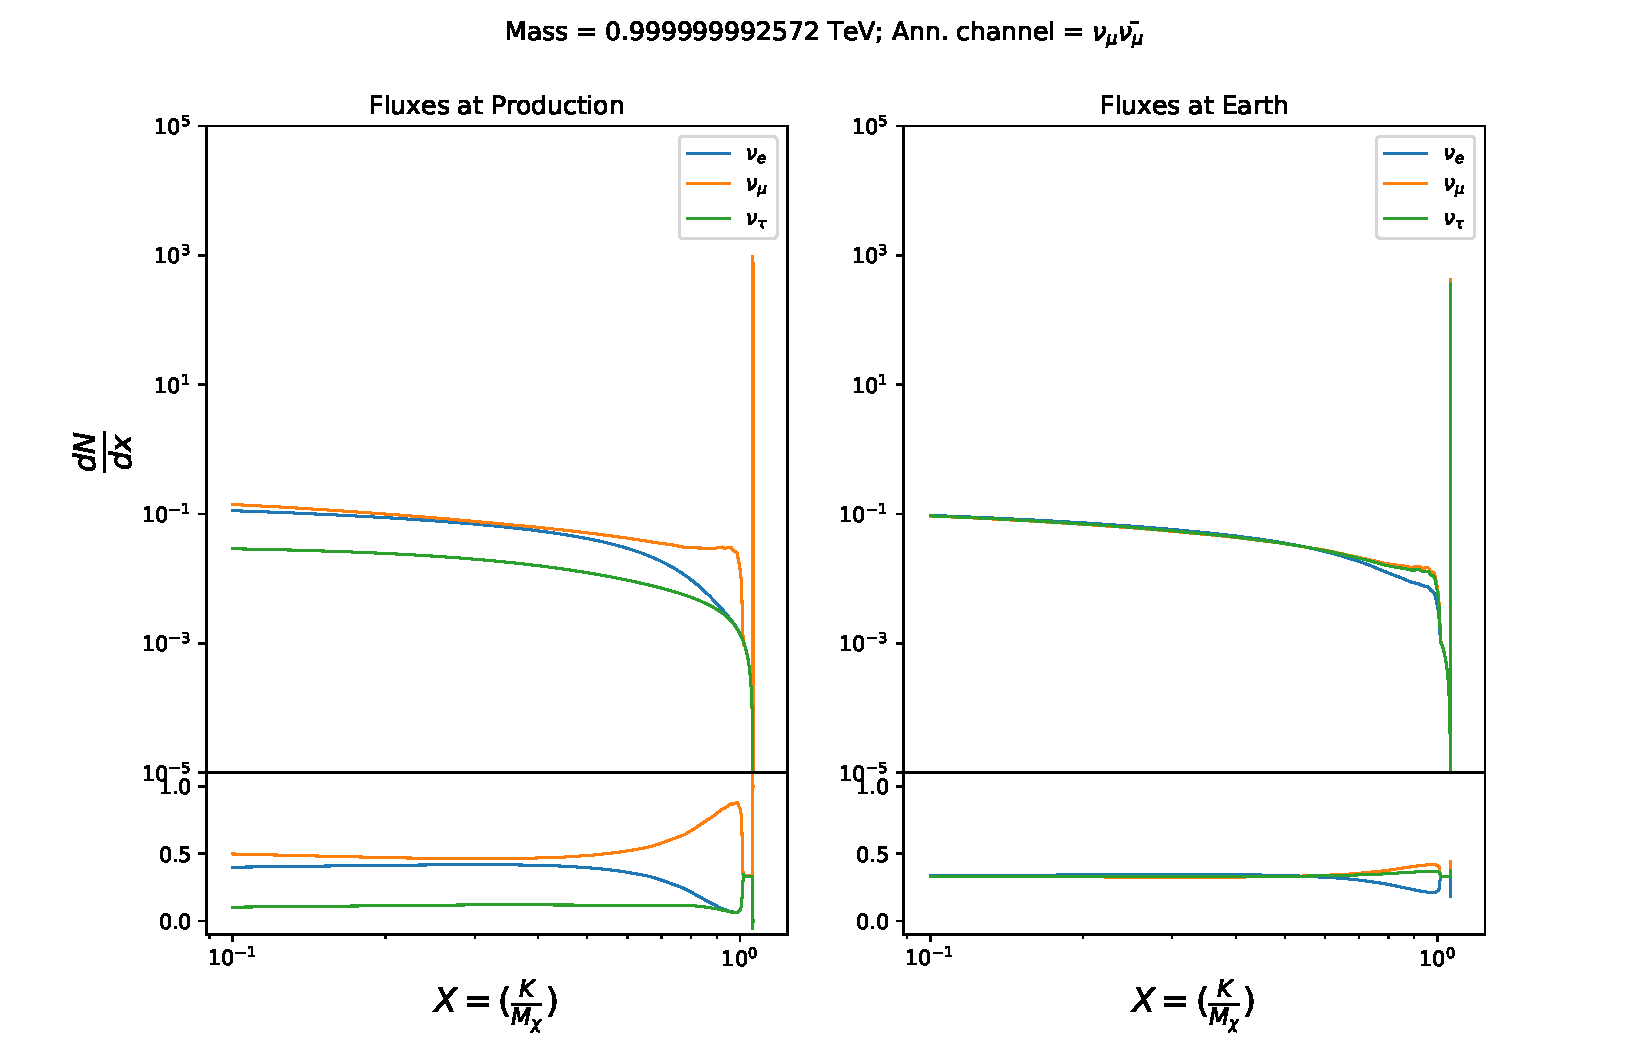
\includegraphics[clip, trim=1cm 0cm 2.5cm 1cm, scale=0.279]{figures/ic_DM/nu_spectra_numunumu_1.0000TeV.pdf}} \\

        \rotatebox[origin=c]{90}{1 PeV} &
        \raisebox{-.5\height}{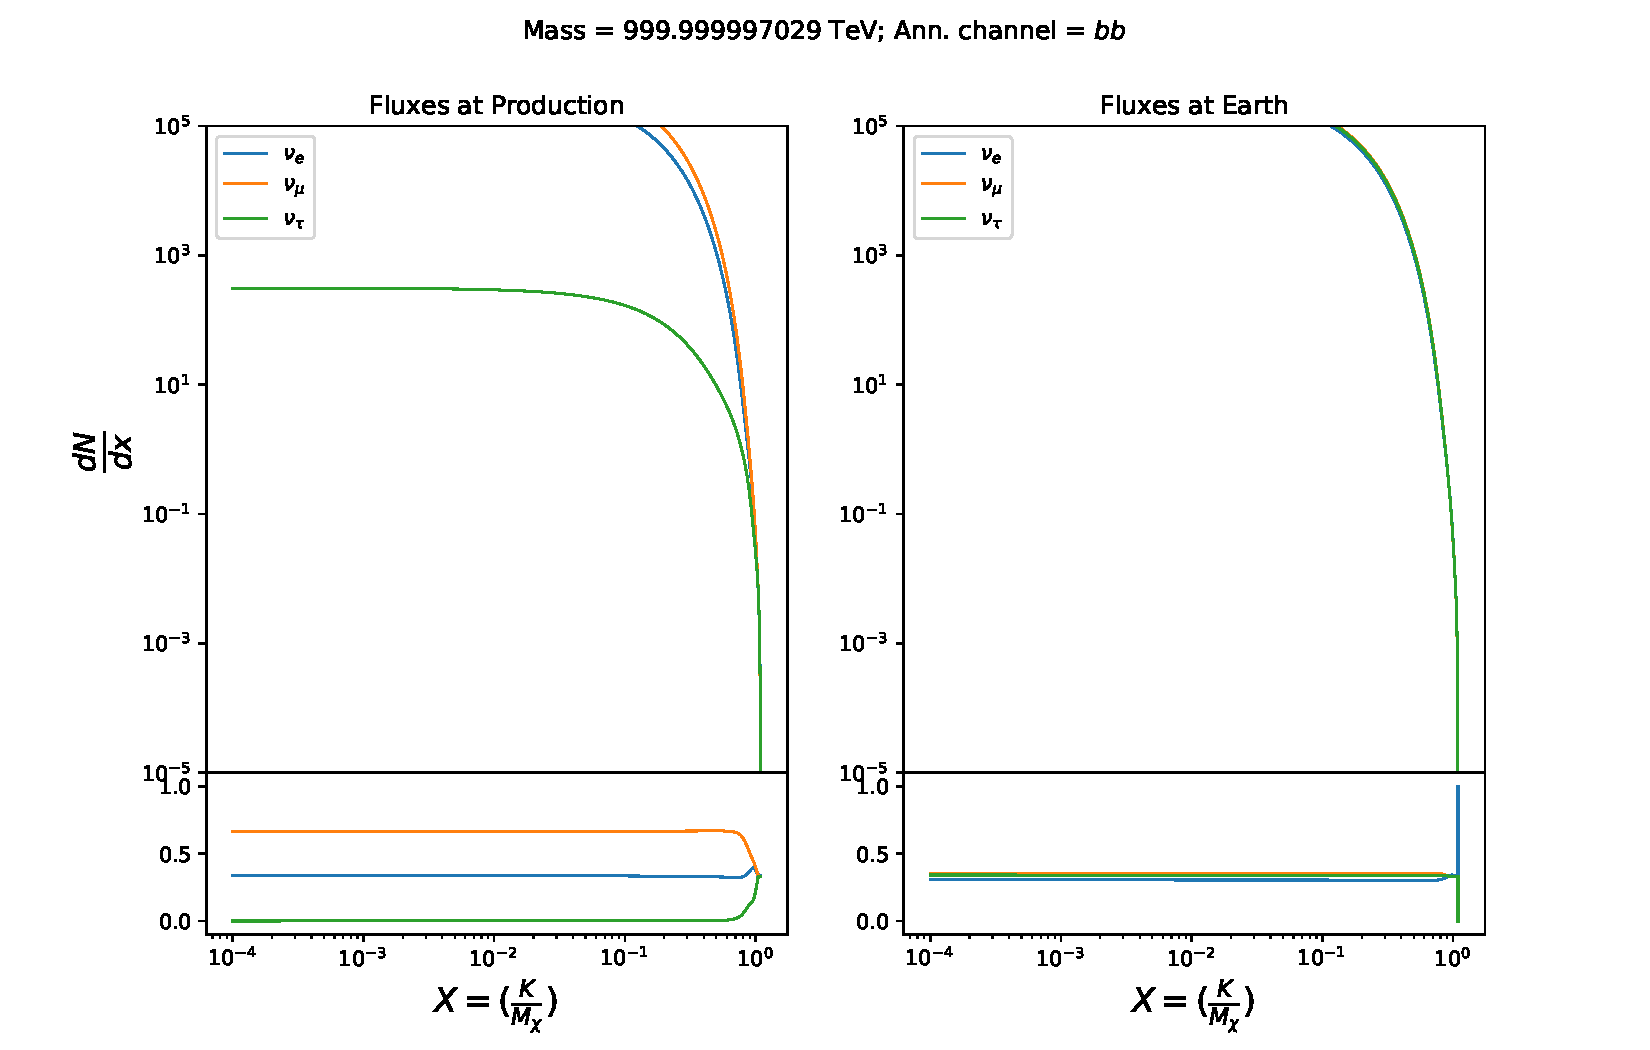
\includegraphics[clip, trim=1cm 0cm 2.5cm 1cm, scale=0.279]{figures/ic_DM/nu_spectra_bb_1000.0000TeV.pdf}} &
        \raisebox{-.5\height}{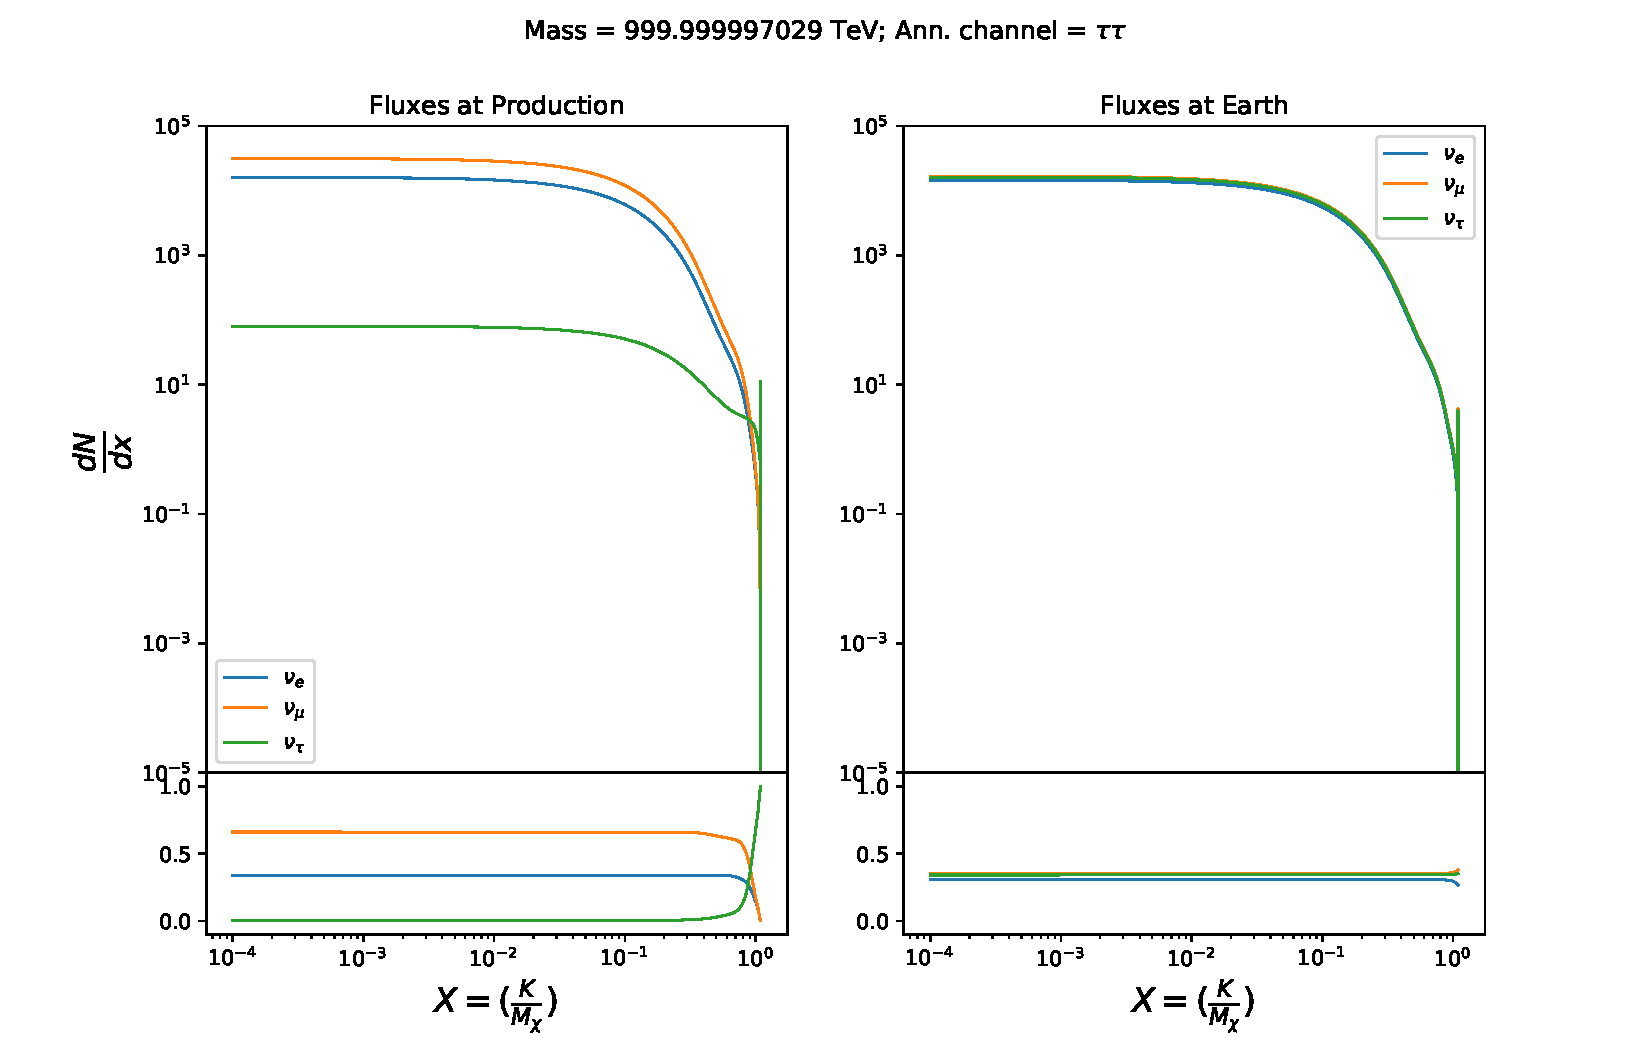
\includegraphics[clip, trim=1cm 0cm 2.5cm 1cm, scale=0.279]{figures/ic_DM/nu_spectra_tautau_1000.0000TeV.pdf}} &
        \raisebox{-.5\height}{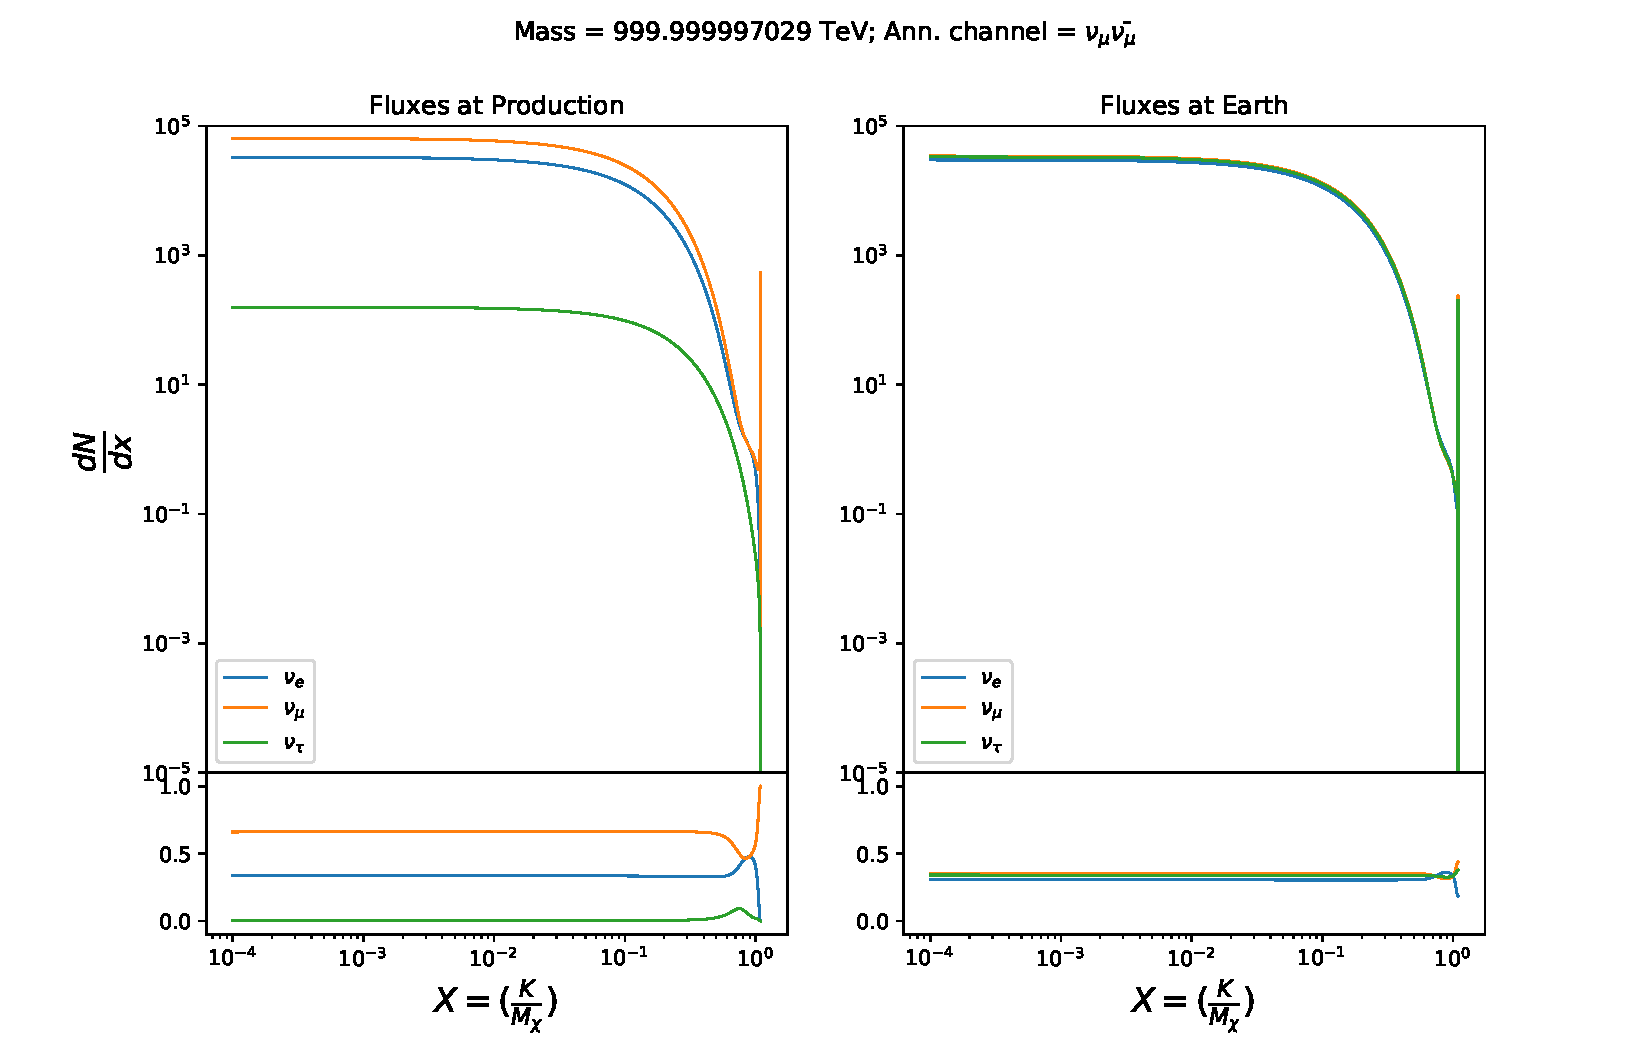
\includegraphics[clip, trim=1cm 0cm 2.5cm 1cm, scale=0.279]{figures/ic_DM/nu_spectra_numunumu_1000.0000TeV.pdf}} \\

        \rotatebox[origin=c]{90}{1 EeV} &
        \raisebox{-.5\height}{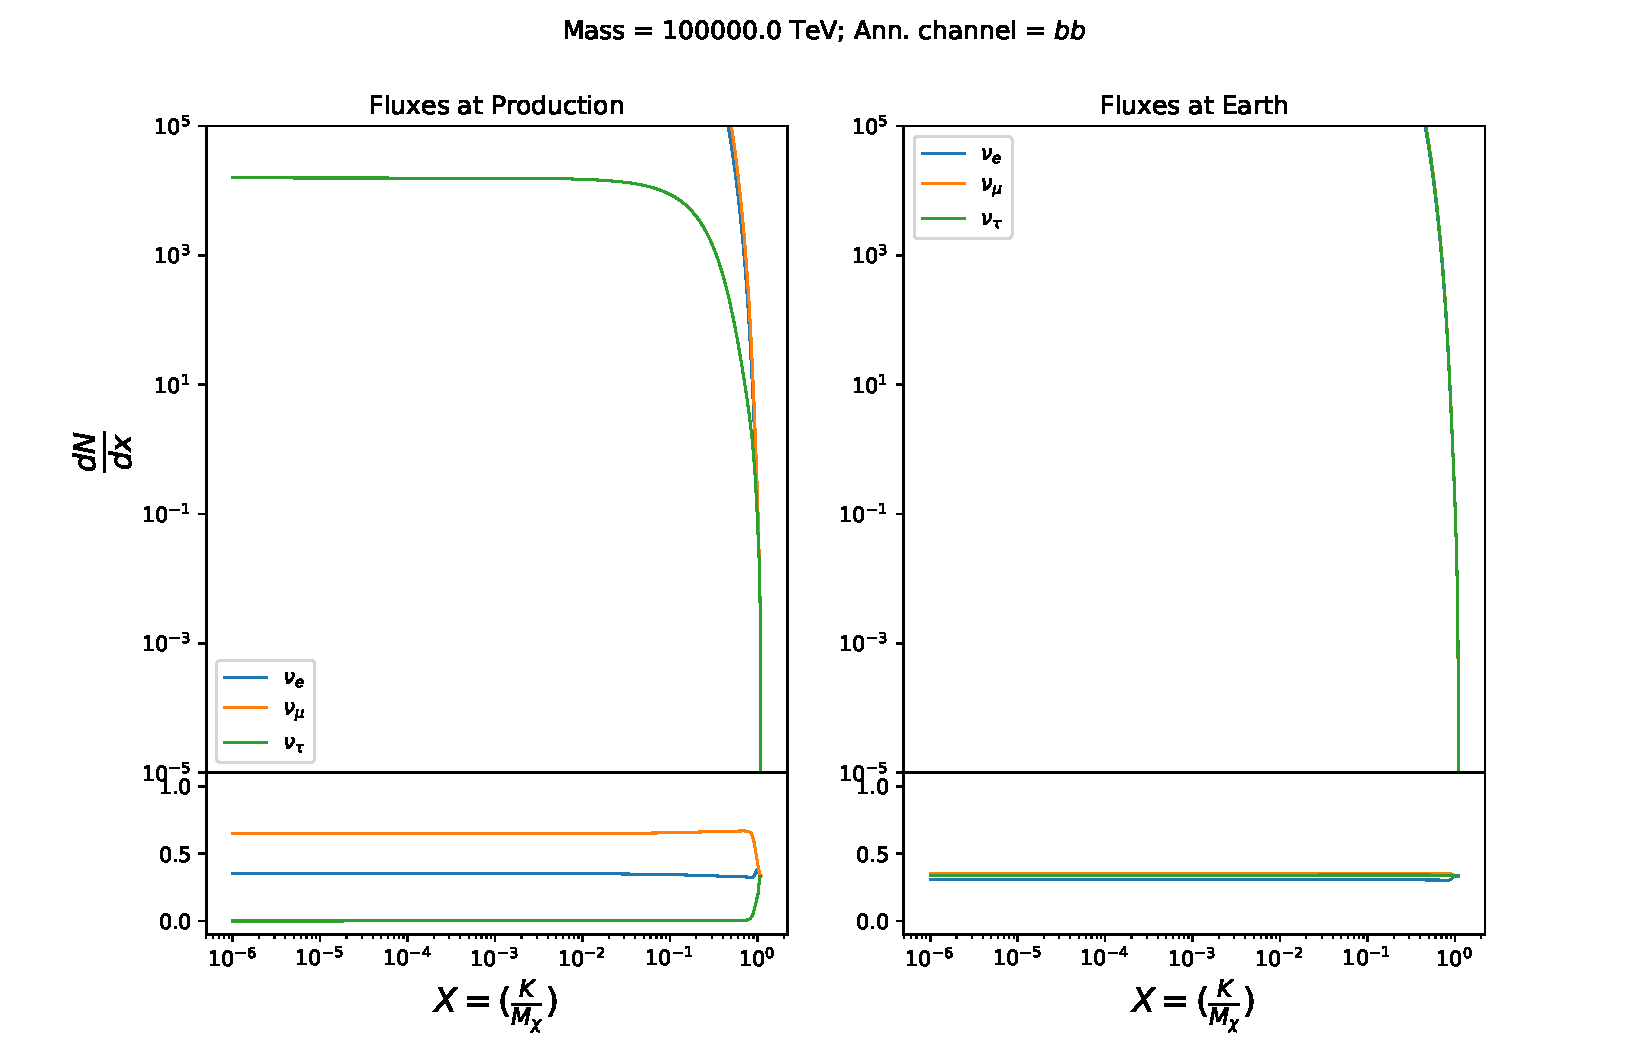
\includegraphics[clip, trim=1cm 0cm 2.5cm 1cm, scale=0.279]{figures/ic_DM/nu_spectra_bb_100000.0000TeV.pdf}} &
        \raisebox{-.5\height}{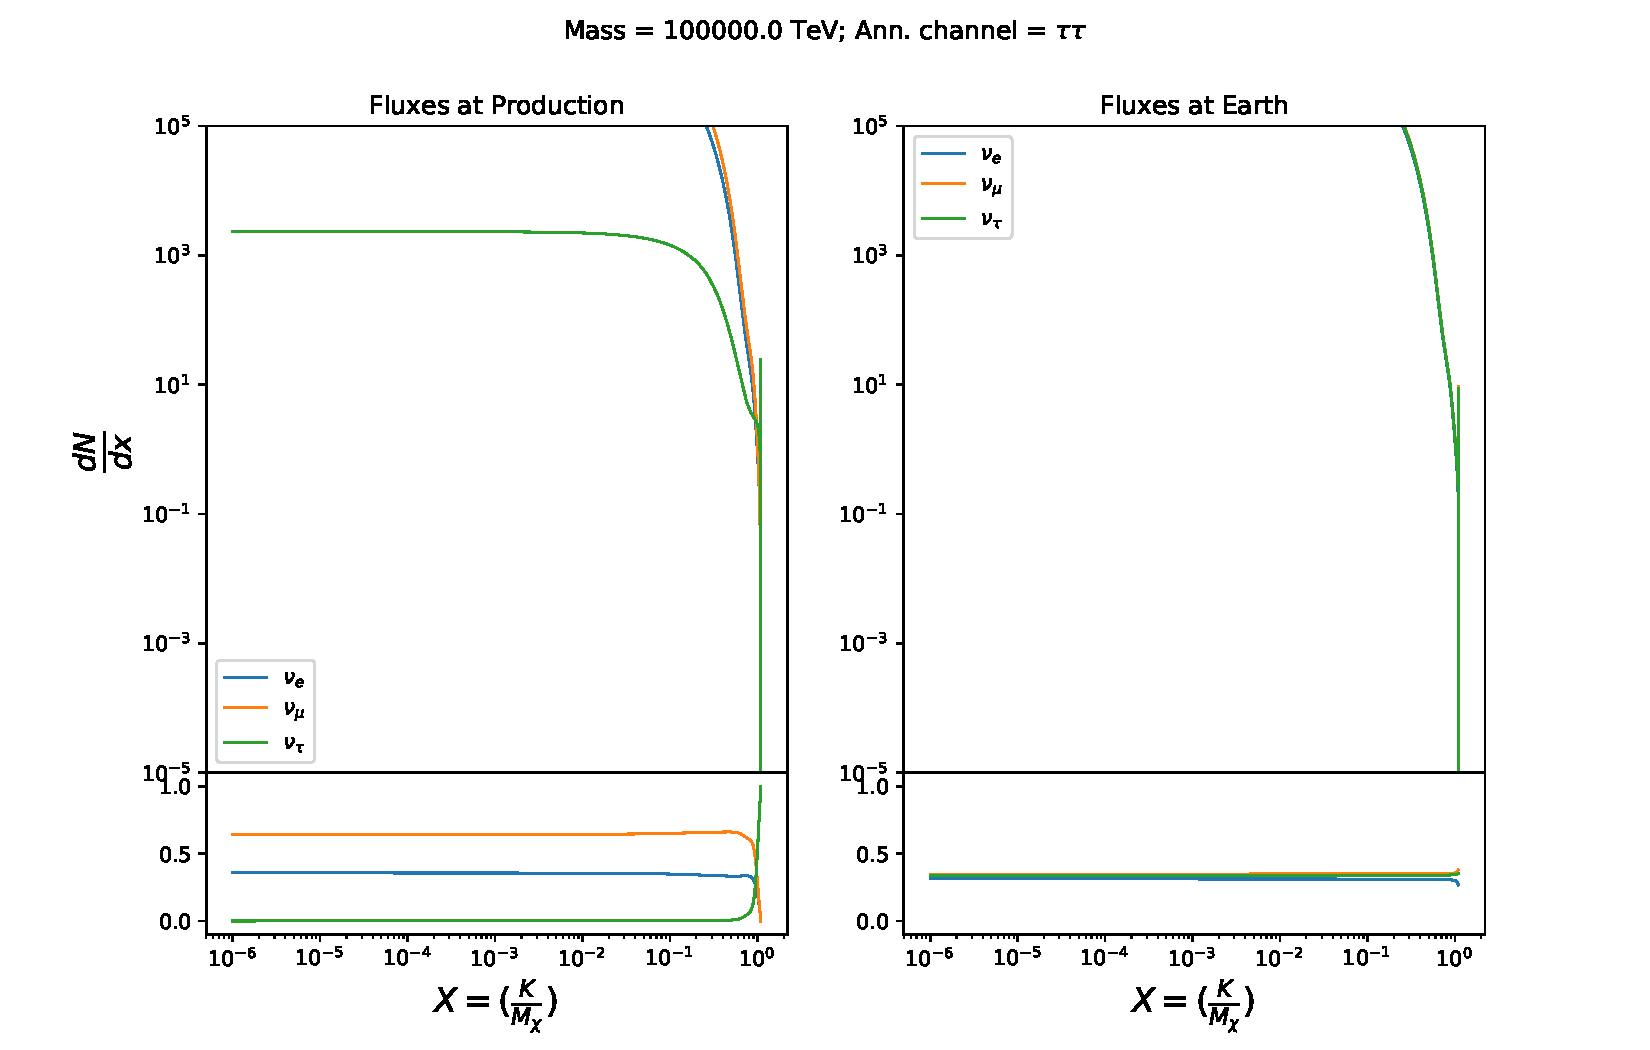
\includegraphics[clip, trim=1cm 0cm 2.5cm 1cm, scale=0.279]{figures/ic_DM/nu_spectra_tautau_100000.0000TeV.pdf}} &
        \raisebox{-.5\height}{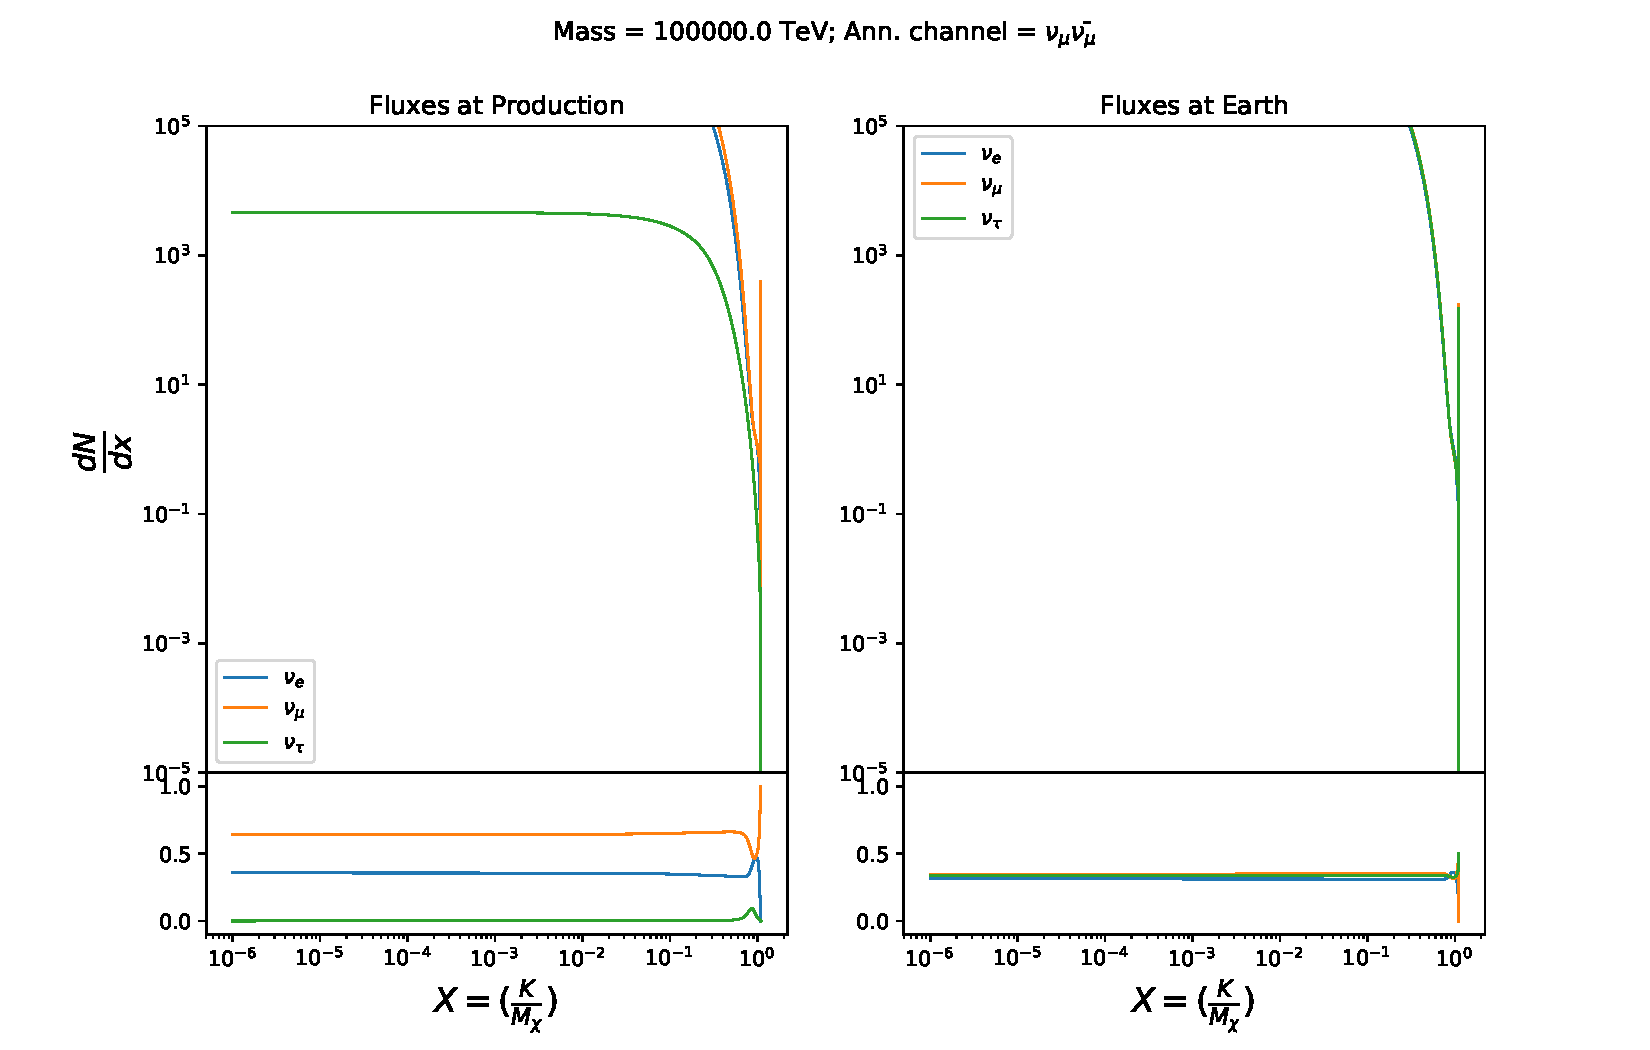
\includegraphics[clip, trim=1cm 0cm 2.5cm 1cm, scale=0.279]{figures/ic_DM/nu_spectra_numunumu_100000.0000TeV.pdf}} \\
    \end{tabular}
    \caption{Neutrino spectra at production (left panels) and after oscillation at Earth (right panels). Blue, orange, and green lines are the $\nu_e$, $\nu_\mu$, and $\nu_\tau$ spectra respectively. Top panels show the spectra in $\frac{dN}{dE}$. Lower panels plot the flavor ratio to $\nu_e + \nu_\mu + \nu_\tau$. SM annihilation channels \parpar{b}, \parpar{\tau}, and \parpar{\nu_\mu} are shown for $M_\chi =$ 1 Pev, TeV, and EeV.}\label{fig:icDM_osc_dm}
}
\end{figure}
\end{landscape}